%! Author = sriadityavedantam
%! Date = 4/7/26

\section{Affine Varieties}

Let $\kk = \bar{\kk}$, as in an algebraic closure such as $\c$ or $\overline{\mathbb{F}_p}$.
We have already studied how
\[
    \aa^n = \{(a_1,\ldots,a_n) : a_i\in\kk\}.
\]
Here $\aa^1$ is a line, and $\aa^2$ is a plane.

\begin{definition}[Zariski Topology]
    A closed subset of $\aa^n$ in the Zariski topology is a set
    \[
        Z = \{f_i(x_1,\ldots,x_n) = 0 : i\in I\},
    \]
    where $f_i\in\kk[x_1,\ldots,x_n]$ for all $i\in I$.
    We call this the zero set of the family $\{f_i\}_{i\in I}$.
\end{definition}

For example, the Zariski topology in $\aa^1$ consists of:
\begin{enumerate}[label={(\arabic*)}]
    \item $\varnothing$, when $f = 1$, so $\{1 = 0\} = \varnothing$.
    \item Finite sets of points, since
    \[
        f(x) = (x-\alpha_1)^{k_1}\cdots(x-\alpha_s)^{k_s}
    \]
    has finitely many zeros.
    \item All of $\aa^1$, when there are no equations imposed.
\end{enumerate}

Whereas in $\aa^2$:

\begin{figure}[H]
    \centering

    \tikzset{every picture/.style={line width=0.75pt}}

    \colorbox{white}{%
        \color{black}
        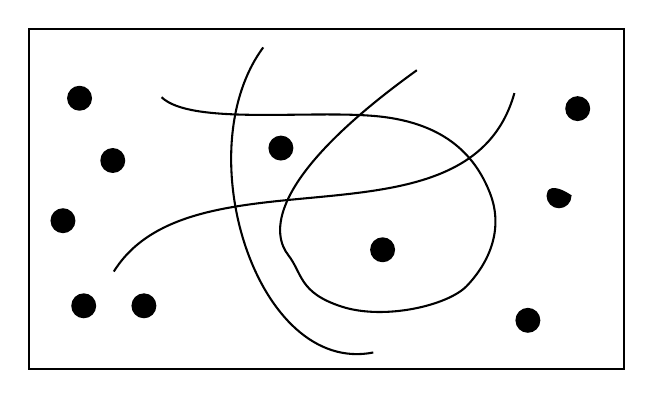
\begin{tikzpicture}[
            x=0.75pt,
            y=0.75pt,
            yscale=-1,
            xscale=1,
            every node/.style={text=black},
            every path/.style={draw=black},
            line width=0.75pt
        ]
            \draw   (188,59) -- (475,59) -- (475,223) -- (188,223) -- cycle ;
            \draw    (252,92) .. controls (265.9,105.34) and (320.79,98.31) .. (354,101) .. controls (387.21,103.69) and (402.74,119.06) .. (410.21,138.14) .. controls (417.67,157.21) and (408,173.7) .. (399,183) .. controls (390,192.3) and (359.35,199.59) .. (338.72,192.87) .. controls (318.08,186.15) and (320,177) .. (313,168) .. controls (306,159) and (300,133) .. (375,79) ;
            \draw    (229,176) .. controls (267,115) and (400,169) .. (422,90) ;
            \draw    (301,68) .. controls (264,118) and (298,226) .. (354,215) ;
            \draw  [color={rgb, 255:red, 0; green, 0; blue, 0 },draw opacity=1][fill={rgb, 255:red, 0; green, 0; blue, 0 },fill opacity=1] (199,151.5) .. controls (199,148.46) and (201.46,146) .. (204.5,146) .. controls (207.54,146) and (210,148.46) .. (210,151.5) .. controls (210,154.54) and (207.54,157) .. (204.5,157) .. controls (201.46,157) and (199,154.54) .. (199,151.5) -- cycle ;
            \draw  [color={rgb, 255:red, 0; green, 0; blue, 0 },draw opacity=1][fill={rgb, 255:red, 0; green, 0; blue, 0 },fill opacity=1] (223,122.5) .. controls (223,119.46) and (225.46,117) .. (228.5,117) .. controls (231.54,117) and (234,119.46) .. (234,122.5) .. controls (234,125.54) and (231.54,128) .. (228.5,128) .. controls (225.46,128) and (223,125.54) .. (223,122.5) -- cycle ;
            \draw  [color={rgb, 255:red, 0; green, 0; blue, 0 },draw opacity=1][fill={rgb, 255:red, 0; green, 0; blue, 0 },fill opacity=1] (207,92.5) .. controls (207,89.46) and (209.46,87) .. (212.5,87) .. controls (215.54,87) and (218,89.46) .. (218,92.5) .. controls (218,95.54) and (215.54,98) .. (212.5,98) .. controls (209.46,98) and (207,95.54) .. (207,92.5) -- cycle ;
            \draw  [color={rgb, 255:red, 0; green, 0; blue, 0 },draw opacity=1][fill={rgb, 255:red, 0; green, 0; blue, 0 },fill opacity=1] (238,192.5) .. controls (238,189.46) and (240.46,187) .. (243.5,187) .. controls (246.54,187) and (249,189.46) .. (249,192.5) .. controls (249,195.54) and (246.54,198) .. (243.5,198) .. controls (240.46,198) and (238,195.54) .. (238,192.5) -- cycle ;
            \draw  [color={rgb, 255:red, 0; green, 0; blue, 0 },draw opacity=1][fill={rgb, 255:red, 0; green, 0; blue, 0 },fill opacity=1] (304,116.5) .. controls (304,113.46) and (306.46,111) .. (309.5,111) .. controls (312.54,111) and (315,113.46) .. (315,116.5) .. controls (315,119.54) and (312.54,122) .. (309.5,122) .. controls (306.46,122) and (304,119.54) .. (304,116.5) -- cycle ;
            \draw  [color={rgb, 255:red, 0; green, 0; blue, 0 },draw opacity=1][fill={rgb, 255:red, 0; green, 0; blue, 0 },fill opacity=1] (447,97.5) .. controls (447,94.46) and (449.46,92) .. (452.5,92) .. controls (455.54,92) and (458,94.46) .. (458,97.5) .. controls (458,100.54) and (455.54,103) .. (452.5,103) .. controls (449.46,103) and (447,100.54) .. (447,97.5) -- cycle ;
            \draw  [color={rgb, 255:red, 0; green, 0; blue, 0 },draw opacity=1][fill={rgb, 255:red, 0; green, 0; blue, 0 },fill opacity=1] (438,139.5) .. controls (438,136.46) and (440.46,134) .. (449,139.5) .. controls (449,142.54) and (446.54,145) .. (443.5,145) .. controls (440.46,145) and (438,142.54) .. (438,139.5) -- cycle ;
            \draw  [color={rgb, 255:red, 0; green, 0; blue, 0 },draw opacity=1][fill={rgb, 255:red, 0; green, 0; blue, 0 },fill opacity=1] (209,192.5) .. controls (209,189.46) and (211.46,187) .. (214.5,187) .. controls (217.54,187) and (220,189.46) .. (220,192.5) .. controls (220,195.54) and (217.54,198) .. (214.5,198) .. controls (211.46,198) and (209,195.54) .. (209,192.5) -- cycle ;
            \draw  [color={rgb, 255:red, 0; green, 0; blue, 0 },draw opacity=1][fill={rgb, 255:red, 0; green, 0; blue, 0 },fill opacity=1] (353,165.5) .. controls (353,162.46) and (355.46,160) .. (358.5,160) .. controls (361.54,160) and (364,162.46) .. (364,165.5) .. controls (364,168.54) and (361.54,171) .. (358.5,171) .. controls (355.46,171) and (353,168.54) .. (353,165.5) -- cycle ;
            \draw  [color={rgb, 255:red, 0; green, 0; blue, 0 },draw opacity=1][fill={rgb, 255:red, 0; green, 0; blue, 0 },fill opacity=1] (423,199.5) .. controls (423,196.46) and (425.46,194) .. (428.5,194) .. controls (431.54,194) and (434,196.46) .. (434,199.5) .. controls (434,202.54) and (431.54,205) .. (428.5,205) .. controls (425.46,205) and (423,202.54) .. (423,199.5) -- cycle ;
        \end{tikzpicture}
    }
\end{figure}

This figure shows some points in the zero set that are of dimension $0$, $1$, and $2$.
This can be very thin if closed and dense if open.

\begin{proposition}{
    Affine varieties give a topology on $\aa^n$.
    In particular:
    \begin{enumerate}[label={(\arabic*)}]
    \item $\varnothing$ is closed, since $\{1 = 0\} = \varnothing$.
    \item $\aa^n$ is closed, corresponding to the empty family of equations.
    \item Arbitrary intersections of closed sets are closed.
    \item Finite unions of closed sets are closed.
    \end{enumerate}
}
    For (3), if $Z_\alpha = \{f_{\alpha,i} = 0 : i\in I_\alpha\}$, then
    \[
        \bigcap_{\alpha\in A} Z_\alpha
    \]
    is again the zero set of the union of all the defining equations.

    For (4), if
    \[
        Z_1 = \{f_{1j} = 0\}
        \quad\text{and}\quad
        Z_2 = \{f_{2k} = 0\},
    \]
    then
    \[
        Z_1\cup Z_2 = \{f_{1j}f_{2k} = 0 \text{ for all } j,k\}.
    \]
\end{proposition}

\begin{lemma*}{
    A curve is non-singular if the dimension of the tangent space is the same as the dimension of the curve.
}
\end{lemma*}

\begin{definition}[Ideal]
    An ideal $I\subset R$ in a commutative ring is a subset such that:
    \begin{enumerate}
        \item $I$ is a subgroup under addition, so if $i_1,i_2\in I$, then $i_1+i_2\in I$.
        \item If $\iota\in R$ and $i\in I$, then $\iota i\in I$.
    \end{enumerate}
\end{definition}

Then $I$ is equal to the set of finite linear combinations of some family of functions $(f_i)$.

\begin{proposition*}{
    If $Z = \{f_i = 0\}$, then $Z = Z(I)$ where $I = (f_i)$.
}
\end{proposition*}

How do we find uniqueness?
Recall the following lemma.

\begin{lemma}{
    Any affine variety in $\aa^n$ can be given by finitely many equations.
}
    Let $Z = \{f_i = 0\}$.
    Then $\kk[x_1,\ldots,x_n]$ is Noetherian, so every ideal is finitely generated.

    The descending chain
    \[
        \{f_1 = 0\}\supseteq \{f_1 = f_2 = 0\}\supseteq \cdots
    \]
    corresponds to the ascending chain
    \[
        (f_1)\subseteq (f_1,f_2)\subseteq \cdots.
    \]
    Since the ring is Noetherian, this chain stabilizes.

    Hence only finitely many equations are needed.

    Uniqueness is expressed canonically by passing to the ideal $I(Z)$.
\end{lemma}

\begin{definition}[Noetherian Space]
    A topological space is Noetherian if and only if it satisfies the descending chain condition on closed subsets.
    That is, for every chain
    \[
        Y_1\supseteq Y_2\supseteq \cdots
    \]
    of closed subsets, there exists an integer $r$ such that
    \[
        Y_r = Y_{r+1} = \cdots.
    \]
\end{definition}

$\aa^n$ is Noetherian.
If
\[
    Y_1\supseteq Y_2\supseteq \cdots,
\]
then
\[
    I(Y_1)\subseteq I(Y_2)\subseteq \cdots
\]
is an ascending chain of ideals in $A = \kk[\reptiln{x}{n}]$.
Since $A$ is a Noetherian ring, this chain of ideals is stationary.
Since for all $i$, $Y_i = Z(I(Y_i))$, the chain of $Y_i$ is stationary as well.

\begin{proposition}{
    In a Noetherian space $X$, every nonempty closed subset $Y$ can be written as a finite union of irreducible closed subsets
    \[
        Y = Y_1\cup\cdots\cup Y_r.
    \]
    If we also require that $Y_i\not\subseteq Y_j$ for $i\neq j$, then the $Y_i$ are uniquely determined.
    These are called the irreducible components of $Y$.
}
    Let $\Epsilon$ be the set of nonempty closed subsets of $X$ which cannot be written as a finite union of irreducible closed subsets.

    If $\Epsilon$ is nonempty, then since $X$ is Noetherian, it contains a minimal element, say $Y$.

    Then $Y$ is not irreducible, by definition of $\Epsilon$.
    Thus
    \[
        Y = Y'\cup Y'',
    \]
    where $Y'$ and $Y''$ are proper closed subsets of $Y$.

    By minimality of $Y$, each of $Y'$ and $Y''$ can be written as a finite union of irreducible closed subsets.
    This gives a decomposition of $Y$, a contradiction.

    Hence every nonempty closed subset can be written as a finite union of irreducible closed subsets.

    Now assume
    \[
        Y = Y_1\cup\cdots\cup Y_r = Y_1'\cup\cdots\cup Y_s',
    \]
    where all $Y_i$ and $Y_j'$ are irreducible, and no one contains another.

    Since
    \[
        Y_1' \subseteq Y_1\cup\cdots\cup Y_r,
    \]
    and $Y_1'$ is irreducible, we must have $Y_1'\subseteq Y_i$ for some $i$.
    Similarly, $Y_i\subseteq Y_j'$ for some $j$.
    By the non-containment assumption, this forces equality.

    Proceeding by induction on the number of components gives uniqueness.
\end{proposition}

\begin{definition}
    Suppose $R$ is a commutative ring with $1$.
    Then
    \[
        \sqrt{I} = \{f\in R : \exists k\geq 1 \text{ such that } f^k\in I\}.
    \]
\end{definition}

\begin{lemma*}{
    $\sqrt{I}$ is an ideal.
}
\end{lemma*}

\begin{theorem}[Hilbert's Nullstellensatz]{
    Let $\aa$ be an ideal in $A = \kk[x_1,\ldots,x_n]$, and let $f\in A$ be a polynomial that vanishes at all points of $Z(\aa)$.
    Then $f^r\in \aa$ for some integer $r>0$.
}
This proof will consult many different theorems, including a paper by Daniel Allcock \cite{allcock}.
\end{theorem}

\subsection{Hilbert's Nullstellensatz}

See \cite{allcock}.

\begin{theorem*}{
    Let $\kk$ be a field and let $\ff$ be a field extension that is finitely generated as a $\kk$-algebra.
    Then $\ff$ is algebraic over $\kk$.
}
\end{theorem*}

\begin{definition}[Algebra]
    An algebra over a field is a vector space equipped with a bilinear product.
\end{definition}

\begin{definition}[Bilinear]
    A bilinear product satisfies distributivity and compatibility with scalar multiplication in each variable.
\end{definition}

\begin{theorem}{
    Suppose $\kk$ is infinite and $\ff = \kk(x)$.
    If $f_1,\ldots,f_m\in\ff$, then the $\kk$-algebra $A$ generated by them is strictly smaller than $\ff$.
}
To see this, choose $c\in\kk$ away from the poles of the rational functions $f_i$.
Then no element of $A$ can have a pole at $c$, so
\[
    \frac{1}{x-c}\notin A.
\]
Thus $A$ is strictly smaller than $\ff$.
\end{theorem}

\begin{definition}[Pole]
    A pole of a rational function is a value where the denominator is $0$.
\end{definition}

\begin{theorem}{
    Assume $\ff$ is transcendental over $\kk$.
    Then $\ff$ is not finitely generated as a $\kk$-algebra.
}
Assume toward a contradiction that $\ff$ is finitely generated as a $\kk$-algebra.
First suppose $\ff$ has transcendence degree $1$.
Then $\ff$ contains a subfield $\kk(x)$ and is algebraic over $\kk(x)$.
Finite generation then implies that $\ff$ has finite dimension over $\kk(x)$.
Choose a basis $e_1,\ldots,e_\ell$ such that
\[
    e_{i}e_j = \sum_k \frac{a_{ijk}(x)}{b_{ijk}(x)}e_k,
\]
with $a_{ijk},b_{ijk}\in\kk[x]$.
Let $f_0 = 1$ be among the generators, and write
\[
    f_i = \sum_j \frac{c_{ij}(x)}{d_{ij}(x)}e_j,
\]
with $c_{ij},d_{ij}\in\kk[x]$.
Then any element $a\in A$ is a $\kk$-linear combination of products of the generators.
Expanding in the basis shows that denominators come only from finitely many $b$'s and $d$'s.
Hence there exists an irreducible polynomial in $\kk[x]$ whose reciprocal does not lie in $A$.
So $A$ is strictly smaller than $\ff$.
This is a contradiction.
If $\ff$ has transcendence degree greater than $1$, reduce to the transcendence degree $1$ case by choosing an intermediate purely transcendental sub-extension.
\end{theorem}

\begin{definition}[Transcendence Degree]
    The transcendence degree of an extension field $K$ over a field $\ff$, denoted $\tdeg(K/\ff)$, is the size of a maximal algebraically independent subset over $\ff$.
\end{definition}

Thus $\mathbb{Q}(\pi)$ and $\mathbb{Q}(\pi,\pi^2)$ still have transcendence degree $1$.
This is because $\pi^2$ is algebraic over $\mathbb{Q}(\pi)$.

\begin{theorem}[Weak Nullstellensatz]{
    Let $\kk$ be an algebraically closed field.
    Then every maximal ideal in the polynomial ring
    \[
        R = \kk[x_1,\ldots,x_n]
    \]
    has the form
    \[
        (x_1-a_1,\ldots,x_n-a_n)
    \]
    for some $a_1,\ldots,a_n\in\kk$.

    As a consequence, a family of polynomials on $\kk^n$ with no common zero generates the unit ideal of $R$.
}
If $m$ is a maximal ideal of $R$, then $R/m$ is a field finitely generated as a $\kk$-algebra.
By the previous theorem, it is algebraic over $\kk$.
Since $\kk$ is algebraically closed, it follows that $R/m \cong \kk$.
Thus each $x_i$ maps to some $a_i\in\kk$ under the quotient map.
So $m$ contains the ideal
\[
    (x_1-a_1,\ldots,x_n-a_n).
\]
Since this is also maximal, equality holds.

For the second statement, if the given family generated a proper ideal, then that ideal would lie in some maximal ideal.
By the first part, that maximal ideal corresponds to a point in $\kk^n$ where all the polynomials vanish.
This contradicts the assumption that they have no common zero.
\end{theorem}

\begin{theorem}[Hilbert's Nullstellensatz]{
    Suppose $\kk$ is an algebraically closed field and $g,f_1,\ldots,f_m\in R = \kk[x_1,\ldots,x_n]$.
    If $g$ vanishes on the common zero-locus of $f_1,\ldots,f_m$, then some power of $g$ lies in the ideal generated by $f_1,\ldots,f_m$.
}
The polynomials $f_1,\ldots,f_m$ and $x_{n+1}g - 1$ have no common zero in $\kk^{n+1}$.
By the Weak Nullstellensatz, we can write
\[
    1 = p_{1}f_1+\cdots+p_{m}f_m+p_{m+1}(x_{n+1}g-1),
\]
where the $p_i$ are polynomials in $x_1,\ldots,x_{n+1}$.
Now apply the homomorphism
\[
    \kk[x_1,\ldots,x_{n+1}] \to \kk(x_1,\ldots,x_n)
\]
given by
\[
    x_{n+1}\mapsto \frac{1}{g}.
\]
This gives
\[
    1 = p_1\!\left(x_1,\ldots,x_n,\frac{1}{g}\right)f_1+\cdots+p_m\!\left(x_1,\ldots,x_n,\frac{1}{g}\right)f_m.
\]
After multiplying through by a suitable power of $g$ to clear denominators, we obtain the result.
\end{theorem}

\begin{definition}[Locus]
    A locus is the set of all points whose coordinates satisfy a given condition.
\end{definition}

\begin{corollary}[Corollary of Nullstellensatz]{
    There is a one-to-one inclusion-reversing correspondence between algebraic sets in $\aa^n$ and radical ideals of $\kk[x_1,\ldots,x_n]$.
    This correspondence is given by
    \[
        Y \mapsto I(Y)
        \quad\text{and}\quad
        \aa \mapsto Z(\aa).
    \]
    An algebraic set is irreducible if and only if its ideal is prime.
}
    $(\implies)$.
    If $Y$ is irreducible, then $I(Y)$ is prime.
    If $fg\in I(Y)$, then
    \[
        Y\subseteq Z(fg) = Z(f)\cup Z(g).
    \]
    Thus
    \[
        Y = (Y\cap Z(f))\cup (Y\cap Z(g)),
    \]
    where both are closed subsets of $Y$.
    Since $Y$ is irreducible, we must have
    \[
        Y\subseteq Z(f)
        \quad\text{or}\quad
        Y\subseteq Z(g).
    \]
    Thus $f\in I(Y)$ or $g\in I(Y)$.

    $(\impliedby)$.
    Let $\pp$ be a prime ideal, and suppose
    \[
        Z(\pp) = Y_1\cup Y_2.
    \]
    Then
    \[
        \pp = I(Z(\pp)) = I(Y_1\cup Y_2) = I(Y_1)\cap I(Y_2).
    \]
    Since $\pp$ is prime, it follows that $\pp = I(Y_1)$ or $\pp = I(Y_2)$.
    Hence
    \[
        Z(\pp) = Y_1
        \quad\text{or}\quad
        Z(\pp) = Y_2,
    \]
    so $Z(\pp)$ is irreducible.
\end{corollary}

\begin{definition}[Prime Ideal]
    A prime ideal is an ideal with the usual prime property:
    if $fg\in \pp$, then $f\in \pp$ or $g\in \pp$.
\end{definition}

\begin{definition}[Irreducible Algebraic Set]
    An algebraic set is irreducible if it cannot be written as the union of two proper algebraic subsets.
\end{definition}

$\aa^n$ is irreducible since it corresponds to the zero ideal in $A$, which is prime.
Let $f$ be an irreducible polynomial in $A = \kk[x,y]$.
Then $f$ generates a prime ideal in $A$, since $A$ is a unique factorization domain.
So the zero set
\[
    Y = Z(f)
\]
is irreducible.
The affine curve is defined by $f(x,y) = 0$.
If $f$ has degree $d$, then $Y$ is a curve of degree $d$.

\begin{definition}[Integral Domain]
    An integral domain is a nontrivial commutative ring in which the product of two nonzero elements is nonzero.
\end{definition}

\begin{definition}[Unique Factorization Domain]
    A unique factorization domain is an integral domain in which every nonunit can be written as a product of irreducible elements, uniquely up to order and multiplication by units.
\end{definition}

\begin{lemma*}{
    A polynomial ring over a field is a UFD.
}
\end{lemma*}

\begin{definition}
    Hence an ideal $I\subset R$ is radical if $\sqrt{I} = I$.
\end{definition}

A counterexample for $\kk = \rr$ is in $\aa^1$:
\[
    Z = \{1 = 0\} = Z((1)) = Z((x^2+1)).
\]
Thus $(x^2+1)\subset \rr[x]$ is radical.
Indeed, if $f^k\in (x^2+1)$, then $f\in (x^2+1)$, since $\rr[x]$ is a UFD and $x^2+1$ is irreducible.

\begin{corollary}{
    We can think of a corollary of the Nullstellensatz as
    \[
        \{\text{radical ideals } J\subset\kk[x_1,\ldots,x_n]\}
        \longleftrightarrow
        \{\text{Zariski closed } S\subset \aa^n_\kk\}.
    \]
}
\end{corollary}